% easier quotes
\newcommand{\gqq}[1]{\glqq#1\grqq}

\section{Präventive Verteidigungsmaßnahmen}

\begin{frame}{Präventive Verteidigungsmaßnahmen}
  \begin{block}{Mehrschichtige Sicherheitsstrukturen}
    \begin{itemize}[<+->]
      \item Sicherheitslücken \textbf{nicht} zu 100\% ausschließbar
      \item Können aber durch mehrschichtige Sicherheitsstrukturen abschwächt werden
      \item Torvalds: \gqq{The only real solution to security is to admit that bugs happen, and then mitigate them by having multiple layers, so if you have a hole in one component, the next layer will catch the issue.} \footnotemark
    \end{itemize}
  \end{block}

  \setbeamerfont{footnote}{size=\tiny}
  \footnotetext{Quelle: http://www.eweek.com/enterprise-apps/linus-torvalds-talks-linux-security-at-linuxcon.html (Besucht am 13.12.2015)}
  \setbeamerfont{footnote}{size=\footnotesize}
\end{frame}

\begin{frame}{Präventive Verteidigungsmaßnahmen}
  \begin{block}{Wie kann man diese mehrschichtige Sicherheitsstrukturen bilden?}
    \begin{itemize}[<+->]
      \item Zugriffskontrolle
      \begin{itemize}[<+->]
        \item AppArmor
        \item SELinux
        \item Grsecurity
      \end{itemize}
      \item Sandboxing
      \begin{itemize}[<+->]
        \item Container
        \item LXC
        \item Docker
      \end{itemize}
    \end{itemize}
  \end{block}
\end{frame}

\begin{frame}{Präventive Verteidigungsmaßnahmen}
  \begin{block}{Zugriffskontrolle}
    \begin{itemize}[<+->]
      \item Zugriffskontrolle kann eine Schicht sein
      \item Zentrale Frage: Wer darf welche Daten lesen, schreiben, ausführen?
      \item Drei grundlegene Modelle:
      \begin{itemize}[<+->]
        \item Mandatory Access Control (MAC)
        \item Discretionary Access Control (DAC)
        \item Role-based Access Control (RBAC)
      \end{itemize}
    \end{itemize}
  \end{block}
\end{frame}

\begin{frame}{Vergleich Zugriffskontrollen}
  \begin{block}{Vergleich}
    \begin{itemize}[<+->]
      \item DAC
      \begin{itemize}[<+->]
        \item Eigentümer entscheidet wer auf das Objekt zugreifen kann
        \item Skaliert schlecht, schwer zu warten
      \end{itemize}
      \item RBAC
      \begin{itemize}[<+->]
        \item Subjekte werden Rollen zugewiesen
        \item Zugriffskontrolle über die Rolle
      \end{itemize}
      \item MAC
      \begin{itemize}[<+->]
        \item Zugriffskontrolle über sog. Labels oder Tags
        \item Skaliert gut, am sichersten
      \end{itemize}
    \end{itemize}
  \end{block}
  \begin{figure}
    \centering
    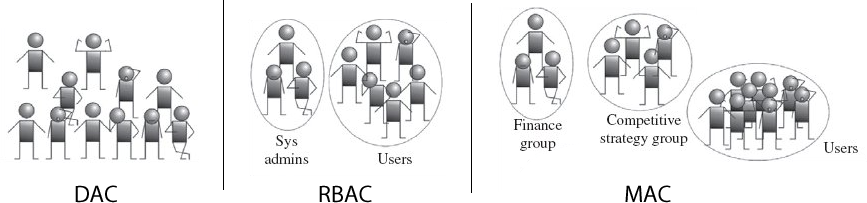
\includegraphics[width=0.75\textwidth]{assets/access_control2}
  \end{figure}
\end{frame}

\begin{frame}{Präventive Verteidigungsmaßnahmen}
  \begin{block}{AppArmor}
    \begin{itemize}[<+->]
      \item Einfache Umsetzung von Mandatory Access Control (MAC)
      \item Schränkt die Rechte von Applikationen ein
      \item Im Vergleich zu SELinux einfache Konfiguration
      \item Schutzziele: Vertraulichkeit, Integrität und Verfügbarkeit
    \end{itemize}
  \end{block}

  \begin{block}{Hätte AppArmor vor Shellshock geschützt?}
    \begin{itemize}[<+->]
      \item Ein Angreifer hätte dennoch Zugriff auf das System erhalten
      \item Rechte wären allerdings stark eingeschränkt
      \item Um schwerwiegenden Schaden auszurichten wären wahrscheinlich weitere Exploits nötig gewesen
    \end{itemize}
  \end{block}
\end{frame}

\begin{frame}{Präventive Verteidigungsmaßnahmen}
  \begin{block}{Sandboxing}
    \begin{itemize}[<+->]
      \item Prinzip: Eine Anwendungen hat keinen Zugriff auf:
      \begin{itemize}[<+->]
        \item eine andere Anwendungen
        \item das System
      \end{itemize}
      \item Vorteile:
      \begin{itemize}[<+->]
        \item Anwendungen isoliert voneinander (in einer Sandbox läuft gewöhnlich genau eine Anwendung)
        \item Schnell \& einfach wiederherstellbar (Disaster Recovery)
        \item Übertragbarkeit auf andere Systeme
        \item Geringer zusatzlicher Ressourcenverbrauch
      \end{itemize}
      \item Einsatz: BIND unter UNIX, Google's Browser Chrome, ...
    \end{itemize}
  \end{block}
\end{frame}

\begin{frame}{Präventive Verteidigungsmaßnahmen}
  \begin{block}{Docker}
    \begin{itemize}[<+->]
      \item Was sind Container?
      \begin{itemize}[<+->]
        \item Ein Set von Prozessen
        \item Isoliert\footnotemark vom Rest der Maschine
        \item Eigene private Resourcen (\textit{namespaces})
        \item Limitierung von Resourcen möglich (\textit{cgroups})
      \end{itemize}
      \item Unterschied zu Virtualisierung?
      \begin{itemize}[<+->]
        \item VM beinhaltet neben der Anwendung auch das Betriebsystem
        \item Container beinhalten nur die Anwendung und sind damit um einiges \gqq{leichter}
      \end{itemize}
      \item Container: Gibt es seit Jahrzehnten
      \item LXC (Linux Container): Gibt es seit Jahren \\
      $\rightarrow$ Docker vereinfacht die Verwendung von LXC
    \end{itemize}
  \end{block}

  \setbeamerfont{footnote}{size=\tiny}
  \footnotetext{Teilen sich den Kernel}
  \setbeamerfont{footnote}{size=\footnotesize}
\end{frame}

\begin{frame}{Präventive Verteidigungsmaßnahmen}
  \begin{block}{Wie sicher ist Docker?}
    \begin{itemize}[<+->]
      \item \gqq{LXC is not yet secure. If I want real security I will use KVM.} Ben Berrangé (LXC Maintainer) 2011\footnotemark
      \item Seit dem hat sich aber einiges getan
      \item Kernel namespaces sind über 5 Jahre alt und damit relativ ausgereift
      \item Docker startet Container mit sehr begrenzten \textit{Capabilities}
      \item Prozesse im Container sollten dennoch nicht als \textit{root} laufen
    \end{itemize}
  \end{block}

  \setbeamerfont{footnote}{size=\tiny}
  \footnotetext{Quelle: https://blog.docker.com/2013/08/containers-docker-how-secure-are-they/ (Besucht am 13.12.2015)}
  \setbeamerfont{footnote}{size=\footnotesize}
\end{frame}

\begin{frame}{Präventive Verteidigungsmaßnahmen}
  \begin{block}{Fazit}
    \begin{itemize}[<+->]
      \item Zwar sind Docker Container inzwischen relativ sicher
      \item Dennoch sollten zusätzliche Sicherheitsschichten verwendet werden \\
      $\rightarrow$ Kombination mit z.B. AppArmor
      \item Ein \textit{sichereres System} druch zusätzliche Sicherheitsschichten entschädigt den erzeugten \textit{Overhead}
    \end{itemize}
  \end{block}
\end{frame}
